\documentclass{bioinfo}
\copyrightyear{2005}
\pubyear{2005}

\usepackage[hyphens]{url}

\begin{document}
\firstpage{1}

\newcommand{\OneReal}{OneChr\_1K}
\newcommand{\SixReal}{SixChr\_1K}
\newcommand{\FullReal}{Full\_1K}
\newcommand{\SixArtiExact}{Chr19\_5K\_0}
\newcommand{\SixArtiNoise}{Chr19\_5K\_10}


\title[MapReduce Clustering]{Scalable Clustering of Genotype Information using MapReduce}
\author[O'Brien \textit{et~al}]{Aidan R O'Brien\,$^{1}$, Fabian A Buske\,$^{2}$ and Denis C. Bauer\,$^1$\footnote{to whom correspondence should be addressed}}
\address{$^{1}$CSIRO, Digital Productivity Flagship, 11 Julius Av, 2113, Sydney, Australia\\
$^{2}$Cancer Epigenetics Program, Cancer Research Division, Kinghorn Cancer Centre, Garvan Institute of Medical Research, 384 Victoria St, 2010, Sydney, Australia}

\history{Received on XXXXX; revised on XXXXX; accepted on XXXXX}

\editor{Associate Editor: XXXXXXX}

\maketitle

\begin{abstract}

\section{Motivation:}
Processing genomic information from whole genome sequence studies pose computational challenges due to the unprecedented data volume generated, which render transitional approaches insufficient. However, by utilising advancements in modern hardware accelerators and data processing we can provide the means for scalable solutions. We therefore aim to provide the interface between standard genomic data formats and advanced and scalable analysis libraries like Mahout. 
\section{Results:}
We achieve an 2-fold speedup by using the scalable k-means MapReduce implementation over the equivalent analysis performed in R, by comparable accuracy. However, the real benefit lies in scaling beyond R's capability to a population-size analysis. We successfully clustered more than 5000 individuals each having more than 15 Million variants. 

\section{Availability:}
Using modern compute paradigms is essential to scale to modern genomic research in an efficient sustainable way. 

\section{Contact:} \href{Denis.Bauer@CSIRO.au}{Denis.Bauer@CSIRO.au}
\end{abstract}

\section{Introduction}

Grouping individuals based on the genomic profile is a commonly performed tasks to identify population structure~\cite{Gao2007} or elucidate different haplotype involvement in diseases susceptibility~\cite{Laitman2013}.  Traditionally both the number of individuals and included genotypes, typically from SNP arrays, were relatively small and libraries in Bioconductor sufficient. However, recent technological advances in whole genome sequencing have made population-scale sequencing feasible. It is hence economical to generate studies with sample sizes currently reserved for larger consortia such as the 1000 genomes project~\cite{1KG2012} or the cancer genome atlas (TCGA)~\cite{TCGA2013}. At the same time, whole genome sequencing enables the inclusion of rare or even somatic mutations in the analysis, increasing the feature space by orders of magnitude. This drastic increase in both sample numbers and features per sample requires a massively parallele approach to data processing. 

As a result of these big data challenges, MapReduce approaches are increasingly being used in bioinformatics (for reviews see~\cite{Zou2013, Qiu2010,Taylor2010}). This is especially the case for sequence analysis tasks, such as read mapping~\cite{Schatz2009}, duplicate removal~\cite{Jourdren2012}, and variant calling~\cite{Langmead2009, McKenna2010} as well as Genome Wide Analysis Study based tasks~\cite{Huang2013, Guo2014}.

%Mention Goolge's population clustering in the intro

At the same time, theoretical computer scientists adapt MapReduce paradigms to cope with the iterative nature of machine learning tasks~\cite{Chu2009}. Specifically, the Mahout project \url{https://mahout.apache.org/} has been developed extensively~\cite{Ranger2007, Owen2011} and was successfully applied in the clinical informatics space~\cite{Dong2013}.

In this paper we link the two areas of parallel machine learning and bioinformatics by providing an interface between Mahout and the standard variant data format, variant call format (VCF)~\cite{1KG2012}, which opens up the application of Mahout's different machine learning algorithms to be applied to genotype-based tasks. 

To demonstrate the capability we cluster variant datasets from the 1000 genomes project to determine population structure as well as ancestry using the k-means clustering algorithm available in Mahout. In the first section we benchmark the performance and accuracy of Mahout's implementations against a standard R based implementation on a reduced version of the data and in the last two sections we investigate how Mahout scales to either more samples or more features per samples.   

%SeqWare~{OConnor2010} Libraries \cite{Doering2008,Schumacher2014,Nordberg2013}


\section*{Results and discussion}

% COMPARISON TO R
\subsection*{Clustering in Mahout uses less memory than in R}
In this section, we compare the runtime between the k-means implementation in R and Mahout for the small \OneReal\ dataset. 
To do this we measured the runtime separately for pre-processing stage as well as the k-means clustering stage itself (see Methods). 
Pre-processing the data to Mahout's sequence files takes 21 minutes, uses 1.8GB physical memory (pmem) and 7.6GB virtual memory (vmem).
Conversely,  pre-processing the data to R's in memory matrix takes 56 minutes, uses 17.7GB pmem and 18GB vmem. 
The size of the Mahout sequence file, which is saved to disk, is 835MB. 
K-means clustering the data, however, is faster with R, using 7s, whereas Mahout takes 10 minutes. See Table~\ref{datasetsTime}. \\
Due to the small number of classifying variants, cluster performance is very poor for both methods, with the best Adjusted Rand Index score for clustering individuals in one of 4 populations (see Methods) being 0.769 for 20 clusters in Mahout and 0.614 with 10 clusters in R (see Table~\ref{datasetsAcc}).

Although the Mahout pipeline is about 25 minutes faster than R's, the actual clustering step takes two orders of magnitude longer. 
This is likely due to the additional overhead involved in setting up the Hadoop nodes, spawning the map and reduce instances, and distributing the data between the instances. 
R on the other hand, already had the data in memory, and only had to process that data. 
In the case of this comparison, the data set is likely too small to truly reap the benefit of Hadoop's MapReduce algorithm. 
The main benefit of Mahout in this scenario is the memory consumption with nearly 10-fold reduction for Mahout compared to R. 


% SCALING UP FEATURES IN MAHOUT
\subsection*{Mahout scales to 15 Million genomic variants}
In this section we demonstrate Mahout's scaling ability by increasing the numbers of features, here variants per sample. 
Including more regions for the similarity calculation will increase the cluster performance, however also increases the memory consumption. 
R therefore was not able to perform the clustering on even the medium sized dataset (\SixReal , 15 Million variants), we hence only report resource consumption and accuracy for Mahout.
On this dataset Mahout's pre-processing takes 325 minutes, with 13GB of physical and 37GB of virtual memory, and the clustering takes 80 minutes.
The clustering accuracy has increased by 35\% to 0.812 with 10 clusters compared to the performance on \OneReal\ for the 4-group-based population task (see Table~\ref{datasetsAcc}).

Utilizing the whole dataset hence would likely increased the performance further. However, on \FullReal\ (38 Million variants) Hadoop returns an 'out-of-memory' error on the name-node before the jobs can even be distributed to the mappers. 
%TODO: is this a correct statement?
It is not possible to use Mahout's standard implementation for this dataset, as the supported Hadoop-setup only allows the communication between nodes with up to 8GB of memory and a scaling beyond that would have been required.

While R does not scale to either of the two orders of magnitude incased datasets, Mahout copes will with up to 15 Million variants. Going beyond this would require an implementation that also paralizes the individual variants as memory directly scales with the size of this feature vector.  


% SCALING UP SAMPLES IN MAHOUT
\subsection*{Mahout scales effortless to an order of magnitude more samples}
In this section we investigate Mahout's ability to scale with more samples.
The resource consumption remains virtually identical between \SixReal\ and the order of magnitude larger dataset \SixArtiExact, which takes 33 minutes, with 6GB of physical and 39GB of virtual memory, and the clustering takes 23 minutes 
The clustering accuracy is 0.812 with 10 clusters.

%TODO: can you think of a less general statement as conclusion
Scaling effortless to massively more samples is the strength of Hadoop, hence compute problems need to be carefully designed to harness this ability.  



\section*{Conclusion}
In this paper we have applied Mahout's k-means clustering to the task of genotype based population and family association. 
We provide an interface from VCF format to Mahout and a toolset to interpret Mahout's clustering output (see Figure 1)
We find that on small datasets the actual clustering stage is two orders of magnitudes slower in Mahout compared to R (10 minutes vs 7 seconds), likely due to the overhead of setting up and co-ordinating the communication between the Hadoop nodes. 
However, increasing either the number of samples or the number of features per sample quickly exceeds the ability of R.
Mahout on the other hand scales effortlessly to five times more samples (5,460) and copes well with 15 Million features per samples.
As memory consumption directly scales with the number of features per sample, we observe that Mahout's standard set-up of Hadoop does not scale to a whole exome dataset (38 Million features per sample).
However, this might be resolved once Mahout moves from MapReduce to a domain-specific language for linear algebraic operations on top of Apache Spark \url{http://spark.apache.org/}.

In conclusion, Mahout offers a scalable out-of-the box solution that is directly applicable to genotype-based clustering for population or family association. 

%This efficient a high performance in-memory map-reduce system has already demonstrated to deliver a  50x speed-up on a whole-genome dataset compared to usual multithreaded approaches, see ADAM~\cite{Massie2013}


\begin{methods}
\section{Methods}
\subsection*{Datasets}
We used variant call format (VCF) files from the 1000 Genomes Project.
These VCF files contain information about the genetic variants between each of the 1092 individuals and a reference genome derived from GRCh37. 
Each of the VCF files are partitioned by chromosome.
Metadata available from the 1000 Genomes Consortium specifies additional attributes for each individual, including population and familial data.\\
To be able to compare with R, we created a subset of the entire human variant dataset by using only variants from chromosome 19 (\OneReal ) where we investigate the correct grouping of the population structure. 
Scaling up using Mahout, we investigate how the accuracy improves when using more variants from the genome with \SixReal\ and \FullReal, which uses chromosome 1-5 in addition to 19 and the full genome, respectively. 
We also investigate whether we can accurately predict the more detailed family association using these datasets. 
In addition, we demonstrate Mahout's scalability by increasing the number of samples in the study to 5,460 by duplicating the original 1092 samples 5 times with zero and 10\% noise levels, i.e. randomly changing 10\% of the genotypes. 
Table~\ref{datasets} contains an overview of the datasets.

\subsection*{Hardware}
We processed the data using a Portable Batch System (PBS) cluster. We allocated one node and 64GB memory for the comparison between Mahout and R.
Each node has eight CPU cores, however both applications run a single thread for pre-processing the data.
%TODO check numbers are correct ?
For the \SixReal\ and \FullReal\ dataset, we ran the job on a PBS cluster of 5 nodes, with twelve CPU cores and 48GB of memory per node.

\subsection*{Pre-processing}
\label{Sec:preprocessing}
Mahout requires Hadoop's `SequenceFiles' as input to its machine learning algorithms. SequenceFiles are binary flat files consisting of key/value pairs. In this case, each of the keys is a
label for an individual. The associated value for each key is a `sparse vector' representing the individual's genomic variants. We use sparse vectors, rather than
dense vectors, to significantly reduce processing time and required disk space. Each sparse vector consists of two separate vectors. An item in the first vector is
effectively a key for an item at the same position in the send vector. The key represents a genomic location, where its value represents the variant. Zero values (positions where there is no variant)
are omitted. Therefore, the fewer variants in an individual's genome, the smaller the sparse vector size. In comparison, `dense vectors' are single arrays that
include every value. Therefore, the size of a dense vector isn't reduced with a large number of non-variants.

The values of the sparse vectors, which, as previously mentioned, represent an individuals genomic variants, are a \texttt{double} java type.
We set the value of each double to the Hamming distance between each variant and the reference genome. Therefore, a value identical to the reference will be 0 (and omitted from the sparse vector),
a heterozygous variant will be 1 and a homozygous variant will be 2.

We wrote a custom `MapReduce' class to convert VCF files to the aforementioned sequence files. This should work on any number of files,
of any file size; limited only by disk space and time. The `map' step creates key value pairs where the primary key is an individual, the secondary key is a variant location, and the value is the variant.
We used a secondary key as this allowed us to implement custom functions to collect and sort the output of each mapper, based on this secondary key. This significantly reduced
the overall processing time. The `reduce' step collects these sorted key/value pairs by primary key (individual ID) and adds the secondary key (location) and value (variant) to a sparse array. The algorithm
saves these sparse arrays and keys to disk in the aforementioned SequenceFile format.   


\subsection*{Mahout K-means clustering}
To cluster the samples from the sequence files, we use Mahout 0.9 in conjunction with Hadoop 2.2.0. 
The clustering steps are the same for each dataset, however, due to the increased feature size we designate more memory to the
YARN containers (a container being the resources allocated to each map or reduce iteration). For the first step, we specify \texttt{k},
the number of clusters. The function \texttt{RandomSeedGenerator.buildRandom} creates a new sequence file containing \texttt{k}
random centroids from the samples sequence file. The sequence file
of samples and the sequence file of centroids serve as the input to \texttt{KMeansDriver.run}, a static Mahout API function that launches
a k-means clustering job on the Hadoop service. 


\subsection*{R K-means clustering}
We use `readVcf' from the R library, `VariantAnnotation', to iteratively read in the VCF file. For each iteration, we convert the data to a matrix and
change the values for each variant to the Hamming distance, as mentioned previously. We then transpose the matrix, so individuals are represented
by rows, and append the matrix to that from the previous iteration. Once the matrix contains all of the variants from the VCF file, we cluster the data
using the `kmeans' algorithm from the `stats' library.



\subsection*{Clustering quality}
We scored the clusters with the Adjusted Rand index~\cite{Hubert1985}. 
This index compares two different cluster sets, here the prediction $X = \{ X_1, X_2, \ldots , X_r \}$ and the annotated data $Y = \{ Y_1, Y_2, \ldots , Y_s \}$, and assigns a value based the overlap between $X$ and $Y$ as captured in a contingency table $\left[n_{ij}\right]$ where each entry $n_{ij}$ denotes the number of objects in common between $X_i$ and $Y_j : n_{ij}=|X_i \cap Y_j|$. 
The Adjusted Rand index is then 
{\tiny
\begin{eqnarray*}
ARI=\frac{\sum_{ij}{{n_{ij}\choose 2}} - \left[ \sum_{i}{{a_i\choose2}} \sum_{j}{{b_i\choose2}} \right] / {n\choose2}}{\frac{1}{2} \left[ \sum_{i}{{a_{i}\choose 2} + \sum_{j}{{b_{j}\choose 2}}} \right] - \left[ \sum_{i}{{a_{i}\choose 2} + \sum_{j}{{b_{j}\choose 2}}} \right] / {n\choose2}} 
\end{eqnarray*}
}
where $a$ and $b$ are the sums over the rows and columns of the contingency table.

The value is zero for independent clusterings and one for identical clusterings. 
We compared the Mahout k-means
clusters and the R k-means clusters to the known clusters based on meta data from the 1000 genome project. For the known clusters,
individuals were partitioned by their super population code (ASN, EUR, AFR, AMR) as well as the 855 families.
%TODO: "also on \chrOnePop" on what dataset did you compare the R performance otherwise ?
%We also compared the Mahout clusters to the
%R clusters for the Chr1 subset data.



\subsection*{Performance}
We recorded the memory usage and run-time from the PBS logs. For the Mahout jobs, we queued separate jobs
for pre-processing and k-means clustering to get an accurate representation of the time and memory requirements for each stage.
For the R job, where we could not easily separate the pre-processing and clustering components, we printed the time between
stages using the function, \texttt{proc.time()}.

\end{methods}

\begin{table}[!t]
\processtable{Datasets used in this study.\label{Tab:01}}
{\begin{tabular}{lrrrrr}\toprule
& individuals  & variants  & population & families & noise\\
& & &groups&& \\\midrule
        \OneReal & 1,092 & 816,115  & 4 & 855 & NA\\
        \SixReal & 1,092 & 15,161,339 & 4 & 855 & NA\\
        \FullReal\ & 1,092 & 38,219,238 & 4 & 855 & NA\\
	\SixArtiExact\ & 5,460 & 816,115 & 4 & 855 & 0 \\ 
	\SixArtiNoise\ & 5,460 & 816,115 & 4 & 855 & 10 \\\botrule
\end{tabular}}{Datasets used in this study}
\end{table}


\begin{table}[!t]
\processtable{Adjusted Rand index (accuracy).\label{Tab:01}}
{\begin{tabular}{lcc}\toprule
Tool, Dataset & accuracy \\\midrule
      R, \OneReal & 0.614  \\ 
        Mahout, \OneReal & 0.605\\
        Mahout, \SixReal & 0.812 \\
        Mahout, \SixArtiExact & 0.600  \\
        Mahout, \SixArtiNoise & 0.140 \\\botrule
\end{tabular}}{Datasets used in this study}
\end{table}

\begin{table*}[!t]
\processtable{Resources consumed.\label{Tab:01}}
{\begin{tabular}{lccccc}\toprule
&&\multicolumn{2}{ c }{Memory (kb)}&\multicolumn{2}{ c }{Time (s)} \\
& Nodes & pmem & vmem  & pre-processing & clustering\\\midrule
         R, \OneReal & 1 & 17,696,940 & 18,000,196 &3,341 & 7\\
        Mahout,\OneReal & 1 & 1,831,160 & 7646232 & 1,255 & 594\\
        Mahout, \SixReal & 5 & 13,036,836 & 36,542,380 & 19,500 & 4820 \\ 
        Mahout, \SixArtiExact & 3 & 5,804,660 & 39,075,548 & 2,024 & 1395 \\\botrule
\end{tabular}}{Datasets used in this study}
\end{table*}


\begin{figure}[!tpb]%figure1
\centerline{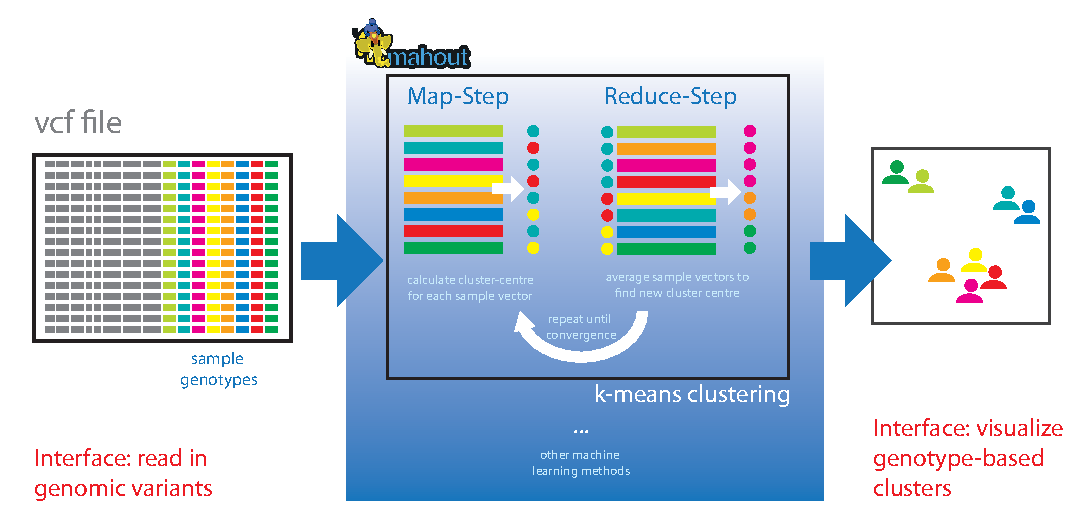
\includegraphics[type=pdf,ext=.pdf,read=.pdf, scale=0.40]{signature}}
        \label{fig:sign}
        \caption{{\bf Illustration of Mahout-based clustering of genotypes.}
      The image shows how the here introduced interface converts the VCF file to a mahout usable vector-based data type. Based on k-means it illustrates how the Map-step procedure groups of vectors by their nearest cluster center and the Reduce-step averages the vectors in each group to find the new value of the updated cluster center. The mahout-produced output is then converted into a visualisation.}

\end{figure}





\section*{Acknowledgement}
A.R.O was funded by the NSW Cancer Institute Big Data Big Impact schema, F.A.B by the National Health and Medical Research Council [1051757] and D.C.B by Commonwealth Scientific and Industrial Research Organisation's Transformational Capability Platform, Science and Industry Endowment Fund and Information Management and Technology Services.
The authors would like to thank Piotr Szul and Gareth Williams for their help with setting up Hadoop on the HPC system.  

\bibliographystyle{natbib}
%\bibliographystyle{achemnat}
%\bibliographystyle{plainnat}
%\bibliographystyle{abbrv}
%\bibliographystyle{bioinformatics}
\bibliography{genotypeClustering}  
\end{document}
